\chapter{Integral} \label{ch3}

Consider a continuous function $f(x)$ defined in $[a, b]$. We want to find the ``antiderivative'' of $f(x)$, i.e. find a function $F(x)$ whose derivative is $f(x)$. In Section \ref{ch3section:motivatingexample}, a motivating example is given to illustrate a use case for such ``antiderivative''. The formal definition of integral is given in Section \ref{ch3sec:integraloffunc}, and the calculation of integral for common functions are given in Section \ref{ch3sec:calculateintegraloffunc}.

\section{A Motivating Example} \label{ch3section:motivatingexample}

Consider the following motivating example where we would like to calculate the area between $y=x^2$ and $y=0$ for $0 \leq x \leq 1$.

\begin{shortbox}
\Boxhead{A Motivating Example}

Consider
\begin{eqnarray}
    y &=& x^2, 0 \leq x \leq 1. \label{ch3eq:motivatingexample}
\end{eqnarray}
A plot of \eqref{ch3eq:motivatingexample} is given in Fig. \ref{ch3fig:motivatingexp}. To obtain the area of the red shape, approximate the red area with the sum of $N$ trapezoids, as shown by the blue dashed curves in Fig. \ref{ch3fig:motivatingexp}.

Q1:  Calculate the sum of the area of the $N$ trapezoids.

Q2: On top of Q1, let $N \rightarrow \infty$ to obtain the area of the red shape.

Q3: Given $0 \leq a \leq 1$, calculate the area of the trapezoids in between two vertical lines $x=0$ and $x=a$.

Q4: Given $0 \leq a \leq 1$, calculate the area of the red in between two vertical lines $x=0$ and $x=a$.

\end{shortbox}

\begin{figure}
\centering
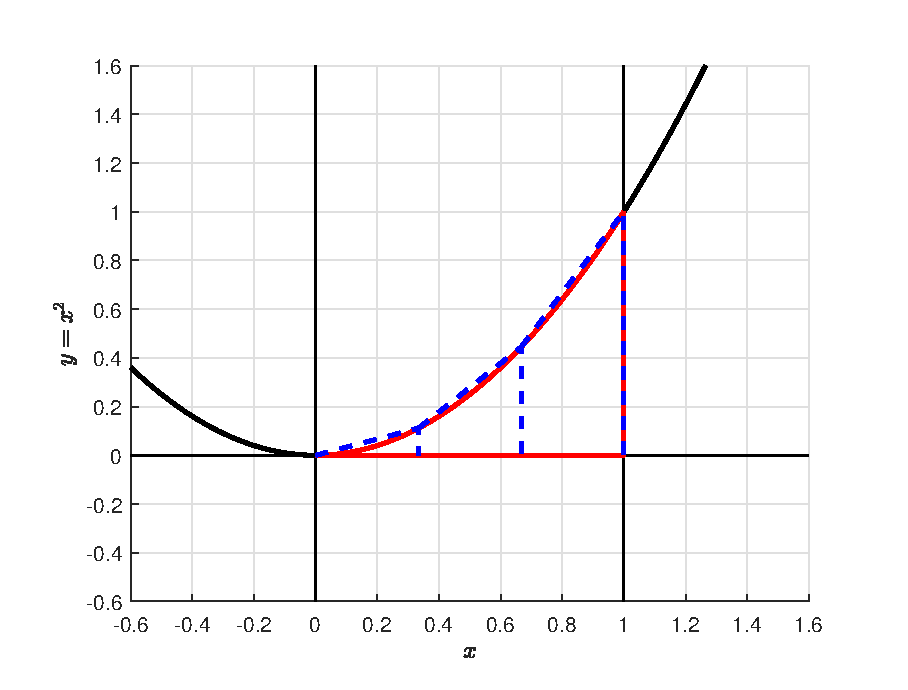
\includegraphics[width=250pt]{chapters/part-1/figures/motivatingexp.eps}
\caption{Plot of \eqref{ch3eq:motivatingexample} and $N=3$ trapezoids.} \label{ch3fig:motivatingexp}
\end{figure}

Notice that in Fig. \ref{ch3fig:motivatingexp}, $N=3$ trapezoids is used in the plot for clearer demonstration. In practice, more trapezoids shall be considered to get a better approximation. We can all agree on that with a larger choice of $N$, a better approximation can be obtained. When $N \rightarrow \infty$, the blue dashed trapezoids approaches the red shape geometrically.

The area of the $i$-th trapezoid can be calculated as follows. (Let the left side smallest triangle be the first trapezoid, and the right side largest trapezoid be the $N$-th trapezoid.)
\begin{eqnarray}
    \Delta x &=& \dfrac{1}{N}, \nonumber \\
    S_i &=& \dfrac{\left((i-1) \Delta x\right)^2 + \left(i \Delta x\right)^2}{2} \Delta x, \nonumber
\end{eqnarray}
where $\Delta x$, $\left((i-1) \Delta x\right)^2$ and $\left(i \Delta x\right)^2$ are the altitude, shorter base and longer base of the $i$-th trapezoid, respectively.

Therefore, the total area of the trapezoids is
\begin{eqnarray}
   s_{T} &=& \sum_{i=1}^{N}S_i \nonumber \\
    &=& \sum_{i=1}^{N} \dfrac{\left((i-1) \Delta x\right)^2 + \left(i \Delta x\right)^2}{2} \Delta x \nonumber \\
    &=& \sum_{i=1}^{N} \dfrac{\left((i-1) \dfrac{1}{N} \right)^2 + \left(i \dfrac{1}{N} \right)^2}{2} \dfrac{1}{N} \nonumber \\
    &=& \dfrac{\sum_{i=1}^{N}\left(2i^2 - 2i + 1\right)}{2N^3}. \label{ch3eq:motivatingexptotalsum}
\end{eqnarray}
Using Table \ref{chi1table:sequencexample}, equation \eqref{ch3eq:motivatingexptotalsum} becomes
\begin{eqnarray}
   s_{T} &=& \dfrac{\dfrac{N(N+1)(2N+1)}{3} - N(N+1) + N}{2N^3} \nonumber \\
    &=& \dfrac{2N^3 + N}{6N^3}. \label{ch3eq:motivatingexptotalsum2}
\end{eqnarray}

Equation \eqref{ch3eq:motivatingexptotalsum2} gives the sum of the area of the trapezoids. For example, substituting $N=3$ into \eqref{ch3eq:motivatingexptotalsum2} gives $s_{T} = 0.3519$. This illustrates the case where 3 trapezoids are used to approximate the area of the red as shown in Fig. \ref{ch3fig:motivatingexp}, and the approximated area is $0.3519$. With larger $N$, a better estimation can be obtained. For example, $N=5$ gives $s_{T} = 0.3400$ and $N=10$ gives $s_{T} = 0.3350$ and $N=20$ gives $s_{T} = 0.3337$. A plot of using $20$ trapezoids to approximate the red area is given in Fig. \ref{ch3fig:motivatingexpN20}. Comparing the two figures \ref{ch3fig:motivatingexp} and \ref{ch3fig:motivatingexpN20}, we can see that $N=20$ is a fairly good approximation and it gives more accurate result than $N=3$.
\begin{figure}
\centering
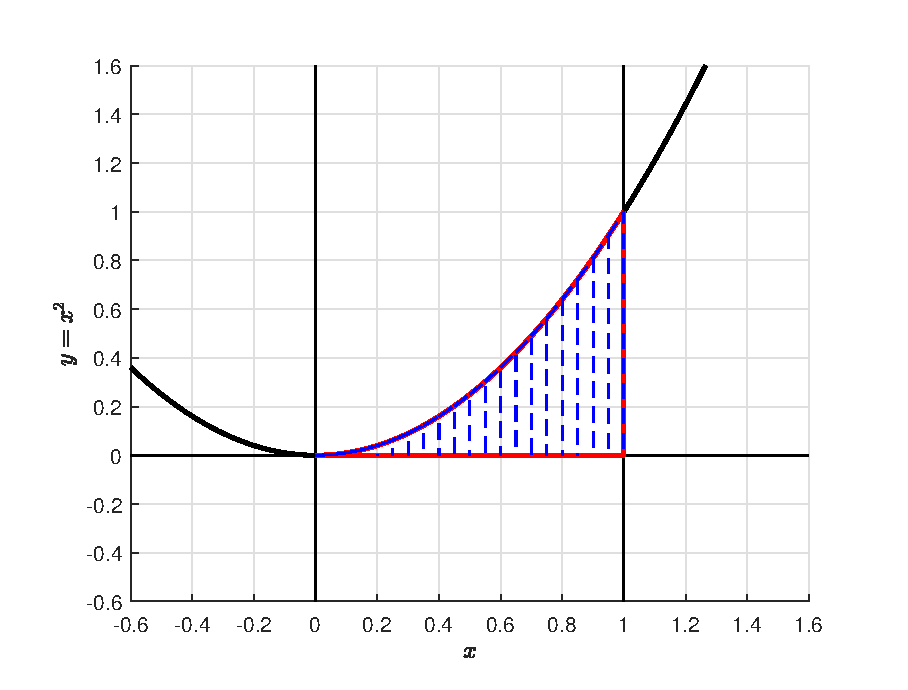
\includegraphics[width=250pt]{chapters/part-1/figures/motivatingexpN20.eps}
\caption{Use $N=20$ trapezoids to approximate the red area.} \label{ch3fig:motivatingexpN20}
\end{figure}

To calculate the precise red area, let $N$ approaches infinity in \eqref{ch3eq:motivatingexptotalsum2} to get
\begin{eqnarray}
    S &=& \lim_{N\rightarrow\infty}\dfrac{2N^3 + N}{6N^3} \nonumber \\
    &=& \lim_{N\rightarrow\infty}\dfrac{2 + \dfrac{1}{N^2}}{6} \nonumber \\
    &=& \dfrac{1}{3}. \nonumber
\end{eqnarray}

The calculation of the trapezoids area in between $x=0$ and $x=a$, $0 \leq a \leq 1$ is tedious but not theoretically difficult. The basic idea is to discuss $a$ in each single trapezoid individually, and finally use a piece-wise function to represent the area. The larger $N$ is, the more segments it will require in the result.

Here we simply use $N=3$ as an example. The result for any arbitrarily large $N$ can be obtained similarly, just with more calculation and probably even support from a computer.

The upper edge of the trapezoids for $N=3$ is given by \ref{ch3eq:motivatingexpN3eq}. It is plotted as the solid blue line in Fig. \ref{ch3fig:motivatingexpN3tra}.
\begin{eqnarray}
    z_{3} &=& \left\{\begin{array}{cc}
        \dfrac{1}{3}x & 0 \leq x \leq \dfrac{1}{3} \\
        x - \dfrac{2}{9} & \dfrac{1}{3} < x \leq \dfrac{2}{3} \\
        \dfrac{5}{3}x - \dfrac{2}{3} & \dfrac{2}{3} < x \leq 1
    \end{array}\right. .\label{ch3eq:motivatingexpN3eq}
\end{eqnarray}

\begin{figure}
\centering
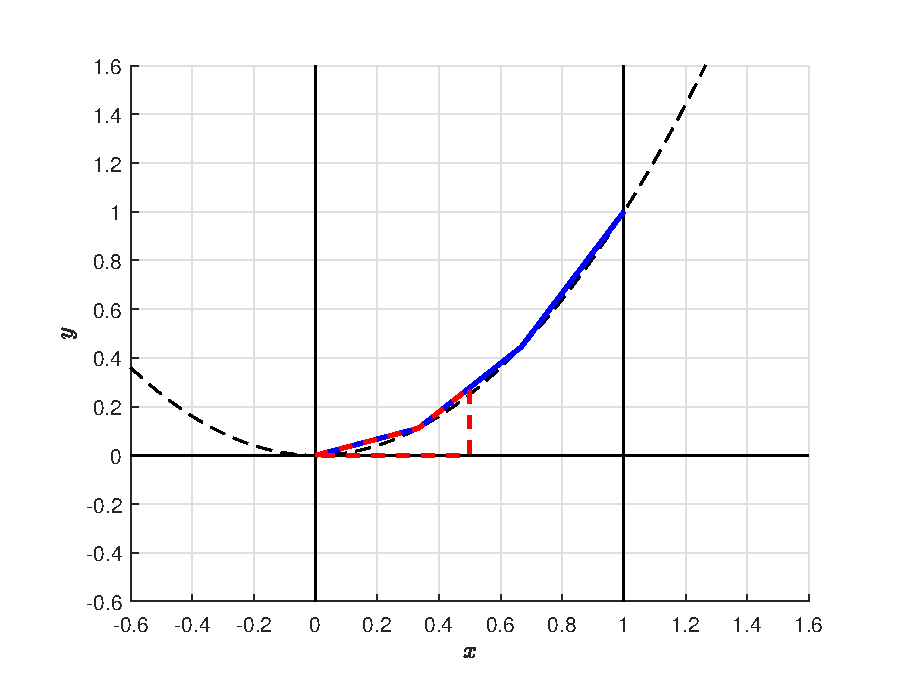
\includegraphics[width=250pt]{chapters/part-1/figures/motivatingexpN3tra.eps}
\caption{Calculation of the area of trapezoids. Variables $N=3$ and $a=0.5$ are used in the plot for demonstration.} \label{ch3fig:motivatingexpN3tra}
\end{figure}

The area of the trapezoids in between $x=0$ and $x=a$ for $N=3$ is given by the red dashed area in Fig. \ref{ch3fig:motivatingexpN3tra}, where $a=0.5$ is used in the plot just for demonstration. The area as a function of $a$ is given as
\begin{eqnarray}
   s_{T}^a &=& \left\{\begin{array}{cc}
        \dfrac{1}{6}a^2 & 0 \leq a \leq \dfrac{1}{3} \\
        \dfrac{1}{2}a^2 - \dfrac{2}{9}a + \dfrac{1}{27} & \dfrac{1}{3} < a \leq \dfrac{2}{3} \\
        \dfrac{5}{6}a^2 - \dfrac{2}{3}a + \dfrac{5}{27} & \dfrac{2}{3} < a \leq 1
    \end{array}\right.. \label{ch3eq:motivatingexpN3eqint}
\end{eqnarray}

The following can be observed from \eqref{ch3eq:motivatingexpN3eq} and \eqref{ch3eq:motivatingexpN3eqint}.
\begin{itemize}
    \item Equation \eqref{ch3eq:motivatingexpN3eqint} is only an approximation to the area in $x=0$, $x=a$, $y=0$ and $y=x^2$. This is because the blue dashed trapezoids are only an approximation to $y=x^2$ given by the black bashed line in Fig. \ref{ch3fig:motivatingexpN3tra}.
    \item By increasing $N$, equation \eqref{ch3eq:motivatingexpN3eqint} gives a better and better approximation. When $N\rightarrow \infty$, the accurate area in $x=0$, $x=a$, $y=0$ and $y=x^2$ can be obtained.
    \item VERY IMPORTANT: Equation \eqref{ch3eq:motivatingexpN3eq} is the derivative of \eqref{ch3eq:motivatingexpN3eqint} for $0 < x < 1$, if replacing the notation ``$a$'' in \eqref{ch3eq:motivatingexpN3eqint} with ``$x$''.
\end{itemize}

The last statement above might be difficult to comprehend and explain, but it can be verified rather easily using \eqref{ch3eq:motivatingexpN3eq} and \eqref{ch3eq:motivatingexpN3eqint}.

Notice that in this motivating example, $y=x^2$, $0 < a < 1$ and $N=3$ are chosen for demonstration purpose without losing generality, thus, this statement shall hold true for any continuous $y=f(x)$ in \eqref{ch3eq:motivatingexample} and any arbitrarily large $N$. We could have chosen $N\rightarrow\infty$ for any $y=f(x)$ to calculate the area in $x=a$, $x=b$, $y=0$ and $y=f(x)$ to get precise (not approximated, since $N\rightarrow\infty$) result.

Furthermore, when $N\rightarrow\infty$, we know that the trapezoids edge given by \eqref{ch3eq:motivatingexpN3eq} will perfectly overlap $y=f(x)$. And we know that \eqref{ch3eq:motivatingexpN3eq} will always be the derivative of the area equation \eqref{ch3eq:motivatingexpN3eqint}. Thus, we can derive \eqref{ch3eq:motivatingexpN3eqint} for the $N\rightarrow\infty$ case by simply looking for a function $F(x)$ whose derivative is $f(x)$. After that, substituting $a$ and $b$ into $F(b)-F(a)$ gives the precise area surrounded by $x = a$, $x = b$, $y=0$ and $y=f(x)$.

An intuitive explanation to this statement is given as follows.

The increment of the area function $F(x)$ from any value $x = a$ to $x = a + \Delta x$ is by definition the area in between $x=a$, $x=a + \Delta x$, $y=0$ and $y=f(x)$. Since $\Delta x$ is very small (in fact, when $N\rightarrow\infty$, $\Delta x \rightarrow 0$), $f(a+\Delta x) \rightarrow f(a)$ and this small area is $f(a)\times\Delta x$. On the other hand, the derivative of $F(x)$ at $x = a$ is defined as this increment $f(a)\times\Delta x$ divided by $\Delta x$. Therefore, the derivative of $F(x)$ at $x=a$ is $f(a)$. Alternatively, we can say \textit{the area function $F(x)$ for $y=f(x)$ is the ``antiderivative'' of $f(x)$}, and in the next section we will meet its official name, the ``integral''.

\section{Integral of a Function} \label{ch3sec:integraloffunc}

In this section, the definitions of \textit{definite integral} and \textit{indefinite integral} are given. As a first step, Riemann integral is introduced. Then, Riemann integral is ``translated'' into the definition of definite integral.

\begin{VF}
\textbf{Definition of Riemann integral}:
\\
\\
Consider a function $f(x)$ defined on interval $[a, b]$. Let $[a, b]$ be split into $N$ consecutive segments whose length are given by $\lambda_1,...,\lambda_N$, with the longest segment's length being $\lambda = \textup{max}\{\lambda_1,...,\lambda_N\}$. Let $x_i$ be a sample randomly taken inside the $i$-th segment.

If for any arbitrarily small $\varepsilon$, there is always such $\delta$ that as long as $\lambda < \delta$,
\begin{eqnarray}
    \left|\sum_{i}f(x_i)\lambda_i - S\right| < \varepsilon, \nonumber
\end{eqnarray}
for a constant $S$, then $S$ is called the Riemann integral of function $f(x)$ on interval $[a, b]$.

\end{VF}

The segment splitting and sampling used in Riemann integral is more general than what Section \ref{ch3section:motivatingexample} has been using. In Section \ref{ch3section:motivatingexample}, we have been assuming even splitting segment $\lambda_i = \lambda_j$ for any two segments, and also determinant sampling in the segment $x_i = \underset{x}{\operatorname{\textup{arg}}} f(x) = \frac{1}{2}\left(f(x_l) + f(x_r)\right)$ where $x_l$, $x_r$ are the left and right boundary of the segment respectively. By assuming continuous function $f(x)$ in Section \ref{ch3section:motivatingexample}, it is guaranteed that such $x_i$ exists. The approach used in Section \ref{ch3section:motivatingexample} is only a special case of Riemann integral, but it would work just fine for most of the cases.

A more intuitive definition of definite integral is given below. The idea is inherited from the motivating example in Section \ref{ch3section:motivatingexample}. It is not as ``strong'' as the Riemann's definition, but should be sufficient for most of the use cases.

\begin{VF}
\textbf{Definition of definite and indefinite integrals in an intuitive manner}:
\\
\\
\noindent

Consider a continuous function $f(x)$ defined on interval $[a, b]$. Let $[a, b]$ be split into $N$ consecutive segments with equal length $\Delta x$. Let $x_i$ be a sample in the $i$-th segment. The \textit{definite integral} of $f(x)$ on interval $[a, b]$ is given by the following equation
\begin{eqnarray}
    S &=& \lim_{\Delta x\rightarrow 0} \sum_i f(x_i)\Delta x, \label{ch3eq:generaldefiniteintegral}
\end{eqnarray}
if the right side limit exists.

In such case, we can rewrite \eqref{ch3eq:generaldefiniteintegral} with the following denotations.
\begin{eqnarray}
    S &=& \int_a^b f(x)dx. \label{ch3eq:generaldefiniteintegral2}
\end{eqnarray}
where $a$ and $b$ are called the lower and upper bound of the integral, respectively. The ``$dx$'' in \eqref{ch3eq:generaldefiniteintegral2} can be taken as $\Delta x \rightarrow 0$.

Equation \eqref{ch3eq:generaldefiniteintegral2} can be solved by finding such $F(x)$ that $\frac{d}{dx}F(x) = f(x)$, and
\begin{eqnarray}
    S = \int_a^b f(x)dx = F(b) - F(a). \label{ch3eq:calculatedefiniteintegral}
\end{eqnarray}
Function $F(x)$ is called the \textit{indefinite integral} of function $f(x)$, and it is denoted by
\begin{eqnarray}
    F(x) &=& \int f(x)dx, \nonumber
\end{eqnarray}
which does not come with the lower and upper bound, and it is often not unique.

\end{VF}

The integral may not exist for some $f(x)$, or at the very least it is impossible to derive an analytical equation $F(x)$ associated with that $f(x)$. It is often easier to derive the derivative of a function, i.e. from $F(x)$ to $f(x)$, than the other way around.

Notice that in the definitions of definite and indefinite integral, continuous $f(x)$ is assumed. For those piece-wise functions that is not continuous at certain values in its range, particular caution is required, for example, to analyze it piece-by-piece considering boundary conditions.

In the case of Riemann integral, the assumption is more relaxed as continuity of $f(x)$ is not required. However, it is still possible that for some $f(x)$, Riemann integral does not exist. For example, Dirichlet function,
\begin{eqnarray}
    D(x) &=& \left\{\begin{array}{cc}
        1 & x \in \mathbb{Q} \\
        0 & \textup{otherwise}
    \end{array}\right.,
\end{eqnarray}
is not continuous or differentiable at any $x$, and it is not Riemann integrable on any interval.

\section{Calculation of the Integral of a Function} \label{ch3sec:calculateintegraloffunc}

Some commonly seen indefinite integral is given in Table \ref{chi3table:commonintegrals}. When calculating indefinite integral, there is always an arbitrary constant $c$ in the result, as the constant in $F(x)$ does not affect the derivative $f(x)$.
\begin{table}
%\noautomaticrules
\tabletitle{Indefinite integral of commonly seen functions.} \label{chi3table:commonintegrals}
\begin{tabular}{lll}
\tch{$f(x)$} & \tch{$F(x) = \int f(x)dx$} & Comments  \\ \hline
$a$ & $ax + c$ & \\
$x^n$ & $\dfrac{1}{n+1}x^{n+1}$ + c & $n\neq -1$ \\
$x^{-1}$ & $\textup{ln}|x| + c$ & $x \neq 0$  \\
$\dfrac{1}{ax+b}$ & $\dfrac{1}{a}\textup{ln}|ax+b| + c$ & $a\neq 0$, $ax+b\neq 0$ \\
$\textup{sin}(x)$ & $-\textup{cos}(x) + c$ & \\
$\textup{cos}(x)$ & $\textup{sin}(x) + c$ & \\
$e^x$ & $e^x + c$ & \\
$\textup{ln}x$ & $x\textup{ln}x - x + c$ & \\
$\dfrac{1}{\sqrt{1-x^2}}$ & $\dfrac{1}{\textup{sin}(x)} + c$ & $|x|<1$\\
$\dfrac{1}{1+x^2}$ & $\dfrac{\textup{cos}(x)}{\textup{sin}(x)}+c$ & \\ \hline
\end{tabular}
\end{table}

If a function is similar to the functions presented in Table \ref{chi3table:commonintegrals}, its indefinite integral might be achievable.

The following rules are commonly used when calculating the integral.
\begin{eqnarray}
    \int f(x) + g(x) &=& \int f(x) dx + \int g(x) dx + c, \nonumber \\
    \int a f(x) dx &=& a \int f(x) dx. \nonumber
\end{eqnarray}

The integral can be calculated by parts as follows.
\begin{eqnarray}
    \int u(x)v^\prime(x)dx = uv - \int u^\prime(x)v(x)dx, \nonumber
\end{eqnarray}
where $u^\prime(x)$, $v^\prime(x)$ are the derivative of $u(x)$ and $v(x)$ respectively. For example, to solve the integral of $f(x)=x\textup{sin}(x)$, let $u(x)=x$, $v^\prime(x)=\textup{sin}(x)$. From Table \ref{chi3table:commonintegrals}, we know that $u^\prime(x)=1$, and $v(x) = -\textup{cos}(x) + c$.
\begin{eqnarray}
    \int f(x)dx &=& \int u(x)v^\prime(x)dx \nonumber \\
    &=& u(x)v(x) - \int u^\prime(x)v(x)dx \nonumber \\
    &=& x\left(-\textup{cos}(x) + c_1\right) - \int \left(-\textup{cos}(x) + c_1\right)dx \nonumber \\
    &=& -x\textup{cos}(x) + \int \textup{cos}(x)dx \nonumber \\
    &=& -x\textup{cos}(x) + \textup{sin}(x) + c. \nonumber
\end{eqnarray}

Inspired by the chain rule of calculation of derivative, the integral can be calculated by substitution as follows.
\begin{eqnarray}
    \int f\left(g(x)\right)dg(x) = \int f\left(g(x)\right)g^\prime(x)dx = F\left(g(x)\right) + c, \nonumber
\end{eqnarray}
where $F(x) = \int f(x)dx$.

In general, the definite integral of a continuous function can be calculated by substituting the upper and lower bound into the indefinite integral and do the following subtraction
\begin{eqnarray}
    \int_a^b f(x)dx = -\int_b^a f(x)dx = F(b) - F(a). \nonumber
\end{eqnarray}
Notice that sometimes $F(b)-F(a)$ is also denoted by $\left.F(x)\right|_a^b$.

As illustrated in the motivating example in Section \ref{ch3section:motivatingexample}, for $a<b$, $\int_a^b f(x)dx$ can be interpreted as the accumulated area between $y=f(x)$ and $y=0$, within boundary $x=a$ and $x=b$.

When $f(x)\geq 0$, $\int_a^b f(x)dx \geq 0$ is the area surrounded by $y=f(x)$, $y=0$, $x=a$ and $x=b$. When $f(x)\leq0$, $\int_a^b f(x)dx \leq 0$ is the negative of the area. Otherwise, $\int_a^b f(x)dx$ is the difference of area above and below $y=0$ as shown in Fig. \ref{ch3fig:explainintegrial}.
\begin{figure}
\centering
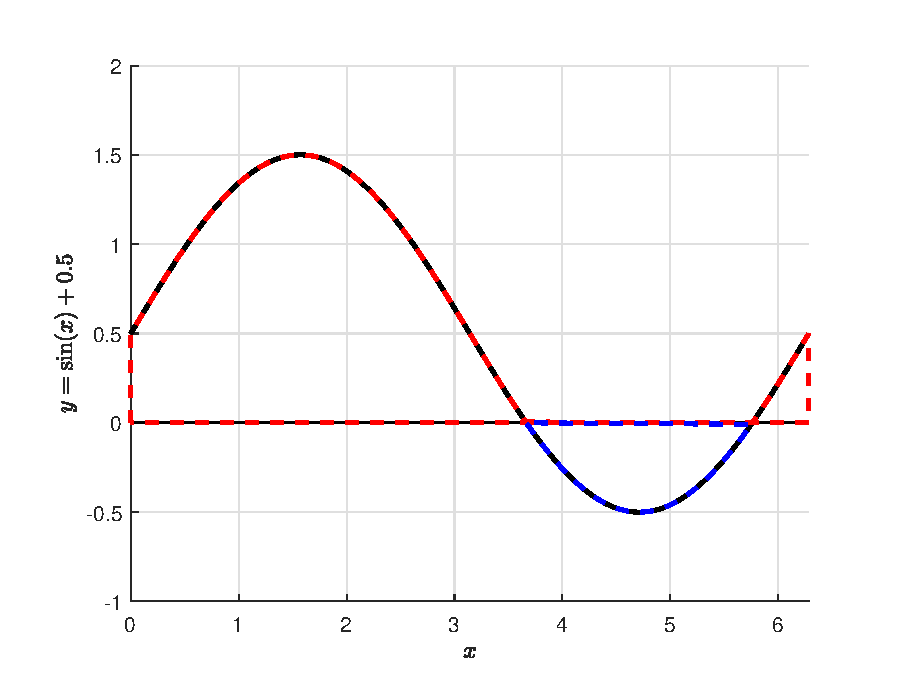
\includegraphics[width=250pt]{chapters/part-1/figures/explainintegrial.eps}
\caption{Plot of $f(x) = \textup{sin}(x) + 0.5$ from $0$ to $2\pi$. The area above $y=0$ is surrounded by the red dashed line, and the area below $y=0$ by the blue dashed line. The definite integral $\int_0^{2\pi}f(x)dx$ in this case is the red area subtracting the blue area.} \label{ch3fig:explainintegrial}
\end{figure}
